% Options for packages loaded elsewhere
\PassOptionsToPackage{unicode}{hyperref}
\PassOptionsToPackage{hyphens}{url}
\PassOptionsToPackage{dvipsnames,svgnames,x11names}{xcolor}
%
\documentclass[
  letterpaper,
  DIV=11,
  numbers=noendperiod]{scrartcl}

\usepackage{amsmath,amssymb}
\usepackage{lmodern}
\usepackage{iftex}
\ifPDFTeX
  \usepackage[T1]{fontenc}
  \usepackage[utf8]{inputenc}
  \usepackage{textcomp} % provide euro and other symbols
\else % if luatex or xetex
  \usepackage{unicode-math}
  \defaultfontfeatures{Scale=MatchLowercase}
  \defaultfontfeatures[\rmfamily]{Ligatures=TeX,Scale=1}
\fi
% Use upquote if available, for straight quotes in verbatim environments
\IfFileExists{upquote.sty}{\usepackage{upquote}}{}
\IfFileExists{microtype.sty}{% use microtype if available
  \usepackage[]{microtype}
  \UseMicrotypeSet[protrusion]{basicmath} % disable protrusion for tt fonts
}{}
\makeatletter
\@ifundefined{KOMAClassName}{% if non-KOMA class
  \IfFileExists{parskip.sty}{%
    \usepackage{parskip}
  }{% else
    \setlength{\parindent}{0pt}
    \setlength{\parskip}{6pt plus 2pt minus 1pt}}
}{% if KOMA class
  \KOMAoptions{parskip=half}}
\makeatother
\usepackage{xcolor}
\setlength{\emergencystretch}{3em} % prevent overfull lines
\setcounter{secnumdepth}{-\maxdimen} % remove section numbering
% Make \paragraph and \subparagraph free-standing
\ifx\paragraph\undefined\else
  \let\oldparagraph\paragraph
  \renewcommand{\paragraph}[1]{\oldparagraph{#1}\mbox{}}
\fi
\ifx\subparagraph\undefined\else
  \let\oldsubparagraph\subparagraph
  \renewcommand{\subparagraph}[1]{\oldsubparagraph{#1}\mbox{}}
\fi

\usepackage{color}
\usepackage{fancyvrb}
\newcommand{\VerbBar}{|}
\newcommand{\VERB}{\Verb[commandchars=\\\{\}]}
\DefineVerbatimEnvironment{Highlighting}{Verbatim}{commandchars=\\\{\}}
% Add ',fontsize=\small' for more characters per line
\usepackage{framed}
\definecolor{shadecolor}{RGB}{241,243,245}
\newenvironment{Shaded}{\begin{snugshade}}{\end{snugshade}}
\newcommand{\AlertTok}[1]{\textcolor[rgb]{0.68,0.00,0.00}{#1}}
\newcommand{\AnnotationTok}[1]{\textcolor[rgb]{0.37,0.37,0.37}{#1}}
\newcommand{\AttributeTok}[1]{\textcolor[rgb]{0.40,0.45,0.13}{#1}}
\newcommand{\BaseNTok}[1]{\textcolor[rgb]{0.68,0.00,0.00}{#1}}
\newcommand{\BuiltInTok}[1]{\textcolor[rgb]{0.00,0.23,0.31}{#1}}
\newcommand{\CharTok}[1]{\textcolor[rgb]{0.13,0.47,0.30}{#1}}
\newcommand{\CommentTok}[1]{\textcolor[rgb]{0.37,0.37,0.37}{#1}}
\newcommand{\CommentVarTok}[1]{\textcolor[rgb]{0.37,0.37,0.37}{\textit{#1}}}
\newcommand{\ConstantTok}[1]{\textcolor[rgb]{0.56,0.35,0.01}{#1}}
\newcommand{\ControlFlowTok}[1]{\textcolor[rgb]{0.00,0.23,0.31}{#1}}
\newcommand{\DataTypeTok}[1]{\textcolor[rgb]{0.68,0.00,0.00}{#1}}
\newcommand{\DecValTok}[1]{\textcolor[rgb]{0.68,0.00,0.00}{#1}}
\newcommand{\DocumentationTok}[1]{\textcolor[rgb]{0.37,0.37,0.37}{\textit{#1}}}
\newcommand{\ErrorTok}[1]{\textcolor[rgb]{0.68,0.00,0.00}{#1}}
\newcommand{\ExtensionTok}[1]{\textcolor[rgb]{0.00,0.23,0.31}{#1}}
\newcommand{\FloatTok}[1]{\textcolor[rgb]{0.68,0.00,0.00}{#1}}
\newcommand{\FunctionTok}[1]{\textcolor[rgb]{0.28,0.35,0.67}{#1}}
\newcommand{\ImportTok}[1]{\textcolor[rgb]{0.00,0.46,0.62}{#1}}
\newcommand{\InformationTok}[1]{\textcolor[rgb]{0.37,0.37,0.37}{#1}}
\newcommand{\KeywordTok}[1]{\textcolor[rgb]{0.00,0.23,0.31}{#1}}
\newcommand{\NormalTok}[1]{\textcolor[rgb]{0.00,0.23,0.31}{#1}}
\newcommand{\OperatorTok}[1]{\textcolor[rgb]{0.37,0.37,0.37}{#1}}
\newcommand{\OtherTok}[1]{\textcolor[rgb]{0.00,0.23,0.31}{#1}}
\newcommand{\PreprocessorTok}[1]{\textcolor[rgb]{0.68,0.00,0.00}{#1}}
\newcommand{\RegionMarkerTok}[1]{\textcolor[rgb]{0.00,0.23,0.31}{#1}}
\newcommand{\SpecialCharTok}[1]{\textcolor[rgb]{0.37,0.37,0.37}{#1}}
\newcommand{\SpecialStringTok}[1]{\textcolor[rgb]{0.13,0.47,0.30}{#1}}
\newcommand{\StringTok}[1]{\textcolor[rgb]{0.13,0.47,0.30}{#1}}
\newcommand{\VariableTok}[1]{\textcolor[rgb]{0.07,0.07,0.07}{#1}}
\newcommand{\VerbatimStringTok}[1]{\textcolor[rgb]{0.13,0.47,0.30}{#1}}
\newcommand{\WarningTok}[1]{\textcolor[rgb]{0.37,0.37,0.37}{\textit{#1}}}

\providecommand{\tightlist}{%
  \setlength{\itemsep}{0pt}\setlength{\parskip}{0pt}}\usepackage{longtable,booktabs,array}
\usepackage{calc} % for calculating minipage widths
% Correct order of tables after \paragraph or \subparagraph
\usepackage{etoolbox}
\makeatletter
\patchcmd\longtable{\par}{\if@noskipsec\mbox{}\fi\par}{}{}
\makeatother
% Allow footnotes in longtable head/foot
\IfFileExists{footnotehyper.sty}{\usepackage{footnotehyper}}{\usepackage{footnote}}
\makesavenoteenv{longtable}
\usepackage{graphicx}
\makeatletter
\def\maxwidth{\ifdim\Gin@nat@width>\linewidth\linewidth\else\Gin@nat@width\fi}
\def\maxheight{\ifdim\Gin@nat@height>\textheight\textheight\else\Gin@nat@height\fi}
\makeatother
% Scale images if necessary, so that they will not overflow the page
% margins by default, and it is still possible to overwrite the defaults
% using explicit options in \includegraphics[width, height, ...]{}
\setkeys{Gin}{width=\maxwidth,height=\maxheight,keepaspectratio}
% Set default figure placement to htbp
\makeatletter
\def\fps@figure{htbp}
\makeatother

\KOMAoption{captions}{tableheading}
\makeatletter
\makeatother
\makeatletter
\makeatother
\makeatletter
\@ifpackageloaded{caption}{}{\usepackage{caption}}
\AtBeginDocument{%
\ifdefined\contentsname
  \renewcommand*\contentsname{Table of contents}
\else
  \newcommand\contentsname{Table of contents}
\fi
\ifdefined\listfigurename
  \renewcommand*\listfigurename{List of Figures}
\else
  \newcommand\listfigurename{List of Figures}
\fi
\ifdefined\listtablename
  \renewcommand*\listtablename{List of Tables}
\else
  \newcommand\listtablename{List of Tables}
\fi
\ifdefined\figurename
  \renewcommand*\figurename{Figure}
\else
  \newcommand\figurename{Figure}
\fi
\ifdefined\tablename
  \renewcommand*\tablename{Table}
\else
  \newcommand\tablename{Table}
\fi
}
\@ifpackageloaded{float}{}{\usepackage{float}}
\floatstyle{ruled}
\@ifundefined{c@chapter}{\newfloat{codelisting}{h}{lop}}{\newfloat{codelisting}{h}{lop}[chapter]}
\floatname{codelisting}{Listing}
\newcommand*\listoflistings{\listof{codelisting}{List of Listings}}
\makeatother
\makeatletter
\@ifpackageloaded{caption}{}{\usepackage{caption}}
\@ifpackageloaded{subcaption}{}{\usepackage{subcaption}}
\makeatother
\makeatletter
\@ifpackageloaded{tcolorbox}{}{\usepackage[many]{tcolorbox}}
\makeatother
\makeatletter
\@ifundefined{shadecolor}{\definecolor{shadecolor}{rgb}{.97, .97, .97}}
\makeatother
\makeatletter
\makeatother
\ifLuaTeX
  \usepackage{selnolig}  % disable illegal ligatures
\fi
\IfFileExists{bookmark.sty}{\usepackage{bookmark}}{\usepackage{hyperref}}
\IfFileExists{xurl.sty}{\usepackage{xurl}}{} % add URL line breaks if available
\urlstyle{same} % disable monospaced font for URLs
\hypersetup{
  pdftitle={Robby - Homework 2},
  colorlinks=true,
  linkcolor={blue},
  filecolor={Maroon},
  citecolor={Blue},
  urlcolor={Blue},
  pdfcreator={LaTeX via pandoc}}

\title{Robby - Homework 2}
\author{}
\date{}

\begin{document}
\maketitle
\ifdefined\Shaded\renewenvironment{Shaded}{\begin{tcolorbox}[borderline west={3pt}{0pt}{shadecolor}, enhanced, breakable, boxrule=0pt, sharp corners, interior hidden, frame hidden]}{\end{tcolorbox}}\fi

\hypertarget{point-process-homework-2}{%
\section{Point Process Homework 2}\label{point-process-homework-2}}

\hypertarget{problem-1}{%
\subsection{Problem 1}\label{problem-1}}

\hypertarget{part-a.}{%
\subsubsection{Part a.}\label{part-a.}}

\begin{Shaded}
\begin{Highlighting}[]
\FunctionTok{library}\NormalTok{(spatstat)}
\end{Highlighting}
\end{Shaded}

\begin{verbatim}
Loading required package: spatstat.data
\end{verbatim}

\begin{verbatim}
Loading required package: spatstat.geom
\end{verbatim}

\begin{verbatim}
spatstat.geom 3.2-5
\end{verbatim}

\begin{verbatim}
Loading required package: spatstat.random
\end{verbatim}

\begin{verbatim}
spatstat.random 3.1-6
\end{verbatim}

\begin{verbatim}
Loading required package: spatstat.explore
\end{verbatim}

\begin{verbatim}
Loading required package: nlme
\end{verbatim}

\begin{verbatim}
spatstat.explore 3.2-3
\end{verbatim}

\begin{verbatim}
Loading required package: spatstat.model
\end{verbatim}

\begin{verbatim}
Loading required package: rpart
\end{verbatim}

\begin{verbatim}
spatstat.model 3.2-6
\end{verbatim}

\begin{verbatim}
Loading required package: spatstat.linnet
\end{verbatim}

\begin{verbatim}
spatstat.linnet 3.1-1
\end{verbatim}

\begin{verbatim}

spatstat 3.0-6 
For an introduction to spatstat, type 'beginner' 
\end{verbatim}

\begin{Shaded}
\begin{Highlighting}[]
\NormalTok{numata\_pines }\OtherTok{\textless{}{-}}\NormalTok{ spatstat.data}\SpecialCharTok{::}\NormalTok{japanesepines}
\FunctionTok{plot}\NormalTok{(numata\_pines}\SpecialCharTok{$}\NormalTok{x,numata\_pines}\SpecialCharTok{$}\NormalTok{y,}\AttributeTok{xlab=}\StringTok{\textquotesingle{}U\textquotesingle{}}\NormalTok{,}\AttributeTok{ylab=}\StringTok{\textquotesingle{}V\textquotesingle{}}\NormalTok{,}\AttributeTok{main=}\StringTok{\textquotesingle{}Japanese Black Pine Sapling Locations\textquotesingle{}}\NormalTok{)}
\end{Highlighting}
\end{Shaded}

\begin{figure}[H]

{\centering 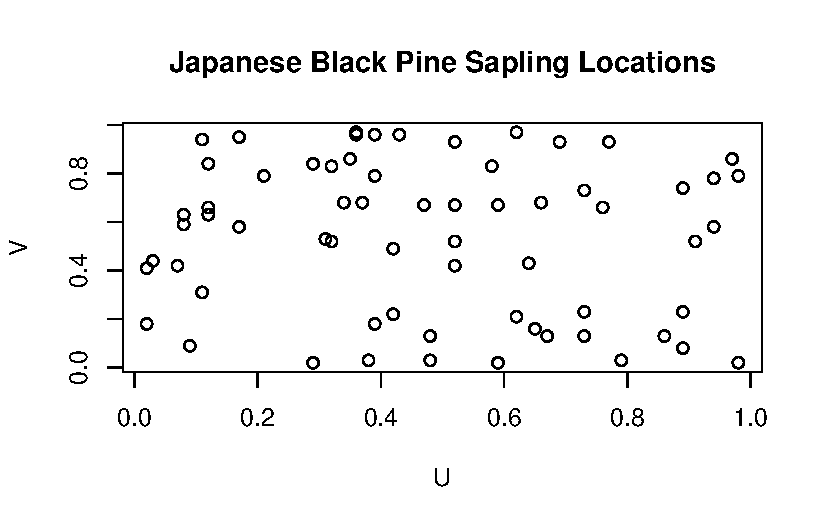
\includegraphics{robby_homework_2_files/figure-pdf/unnamed-chunk-1-1.pdf}

}

\end{figure}

\begin{Shaded}
\begin{Highlighting}[]
\NormalTok{lplot }\OtherTok{\textless{}{-}} \ControlFlowTok{function}\NormalTok{(x, }\AttributeTok{nsim =} \DecValTok{500}\NormalTok{, }\AttributeTok{level =} \FloatTok{0.95}\NormalTok{,}
                  \AttributeTok{correction =} \StringTok{"Ripley"}\NormalTok{, }\AttributeTok{test=}\ConstantTok{FALSE}\NormalTok{, ...) \{}
\NormalTok{  lobs }\OtherTok{\textless{}{-}}\NormalTok{ spatstat.explore}\SpecialCharTok{::}\FunctionTok{Lest}\NormalTok{(x, }\AttributeTok{correction =}\NormalTok{ correction, ...)}


\NormalTok{  win }\OtherTok{\textless{}{-}}\NormalTok{ x}\SpecialCharTok{$}\NormalTok{window}
\NormalTok{  lsim }\OtherTok{\textless{}{-}}\NormalTok{ pbapply}\SpecialCharTok{::}\FunctionTok{pblapply}\NormalTok{(}\DecValTok{1}\SpecialCharTok{:}\NormalTok{nsim, }\AttributeTok{FUN =} \ControlFlowTok{function}\NormalTok{(i) \{}

\NormalTok{    xsim }\OtherTok{\textless{}{-}}\NormalTok{ spatstat.random}\SpecialCharTok{::}\FunctionTok{rpoispp}\NormalTok{(}\AttributeTok{lambda =}\NormalTok{ x}\SpecialCharTok{$}\NormalTok{n, }\AttributeTok{win =}\NormalTok{ win)}
\NormalTok{    spatstat.explore}\SpecialCharTok{::}\FunctionTok{Lest}\NormalTok{(xsim, }\AttributeTok{correction =}\NormalTok{ correction, ...)}
\NormalTok{  \})}

\NormalTok{  r }\OtherTok{\textless{}{-}}\NormalTok{ lobs}\SpecialCharTok{$}\NormalTok{r }\CommentTok{\# get distances}
\NormalTok{  obs }\OtherTok{\textless{}{-}}\NormalTok{ lobs}\SpecialCharTok{$}\NormalTok{iso }\CommentTok{\# get estimated l for observed}
  \CommentTok{\# get estimated l for each simulated data set}
\NormalTok{  sim }\OtherTok{\textless{}{-}} \FunctionTok{sapply}\NormalTok{(lsim, getElement, }\StringTok{"iso"}\NormalTok{)}
  \CommentTok{\# apply the min function to each row  (MARGIN = 1) of sim}
  \CommentTok{\# gets pointwise minimum for simulated data}
  \CommentTok{\# at each distance.  do same for max, quantiles, median}
\NormalTok{  lo }\OtherTok{\textless{}{-}} \FunctionTok{apply}\NormalTok{(sim, }\AttributeTok{MARGIN =} \DecValTok{1}\NormalTok{, }\AttributeTok{FUN =}\NormalTok{ min, }\AttributeTok{na.rm =} \ConstantTok{TRUE}\NormalTok{)}
\NormalTok{  hi }\OtherTok{\textless{}{-}} \FunctionTok{apply}\NormalTok{(sim, }\AttributeTok{MARGIN =} \DecValTok{1}\NormalTok{, }\AttributeTok{FUN =}\NormalTok{ max, }\AttributeTok{na.rm =} \ConstantTok{TRUE}\NormalTok{)}
\NormalTok{  alpha }\OtherTok{\textless{}{-}} \DecValTok{1} \SpecialCharTok{{-}}\NormalTok{ level}
\NormalTok{  qlo }\OtherTok{\textless{}{-}} \FunctionTok{apply}\NormalTok{(sim, }\AttributeTok{MARGIN =} \DecValTok{1}\NormalTok{, }\AttributeTok{FUN =}\NormalTok{ quantile,}
               \AttributeTok{prob =}\NormalTok{ alpha}\SpecialCharTok{/}\DecValTok{2}\NormalTok{, }\AttributeTok{na.rm =} \ConstantTok{TRUE}\NormalTok{)}
\NormalTok{  qhi }\OtherTok{\textless{}{-}} \FunctionTok{apply}\NormalTok{(sim, }\AttributeTok{MARGIN =} \DecValTok{1}\NormalTok{, }\AttributeTok{FUN =}\NormalTok{ quantile,}
               \AttributeTok{prob =} \DecValTok{1} \SpecialCharTok{{-}}\NormalTok{ alpha}\SpecialCharTok{/}\DecValTok{2}\NormalTok{, }\AttributeTok{na.rm =} \ConstantTok{TRUE}\NormalTok{)}
\NormalTok{  med }\OtherTok{\textless{}{-}} \FunctionTok{apply}\NormalTok{(sim, }\AttributeTok{MARGIN =} \DecValTok{1}\NormalTok{, }\AttributeTok{FUN =}\NormalTok{ median, }\AttributeTok{na.rm =} \ConstantTok{TRUE}\NormalTok{)}
  \CommentTok{\# construct empty plot of the right size}
  \FunctionTok{plot}\NormalTok{(}\FunctionTok{range}\NormalTok{(r), }\FunctionTok{c}\NormalTok{(}\FunctionTok{min}\NormalTok{(}\FunctionTok{c}\NormalTok{(lo, obs) }\SpecialCharTok{{-}}\NormalTok{ r, }\AttributeTok{na.rm =} \ConstantTok{TRUE}\NormalTok{),}
                   \FunctionTok{max}\NormalTok{(}\FunctionTok{c}\NormalTok{(hi, obs) }\SpecialCharTok{{-}}\NormalTok{ r, }\AttributeTok{na.rm =} \ConstantTok{TRUE}\NormalTok{)),}
       \AttributeTok{type =} \StringTok{"n"}\NormalTok{,}
       \AttributeTok{xlab =} \StringTok{"distance"}\NormalTok{, }\AttributeTok{ylab =} \StringTok{"L(r) {-} r"}\NormalTok{)}
  \CommentTok{\# plot different statistics with different styles/thickness}
  \FunctionTok{lines}\NormalTok{(r, obs }\SpecialCharTok{{-}}\NormalTok{ r, }\AttributeTok{lwd =} \DecValTok{2}\NormalTok{)}
  \FunctionTok{lines}\NormalTok{(r, lo }\SpecialCharTok{{-}}\NormalTok{ r, }\AttributeTok{lty =} \DecValTok{2}\NormalTok{)}
  \FunctionTok{lines}\NormalTok{(r, hi }\SpecialCharTok{{-}}\NormalTok{ r, }\AttributeTok{lty =} \DecValTok{2}\NormalTok{)}
  \FunctionTok{lines}\NormalTok{(r, qlo }\SpecialCharTok{{-}}\NormalTok{ r, }\AttributeTok{lty =} \DecValTok{1}\NormalTok{)}
  \FunctionTok{lines}\NormalTok{(r, qhi }\SpecialCharTok{{-}}\NormalTok{ r, }\AttributeTok{lty =} \DecValTok{1}\NormalTok{)}
  
\NormalTok{\}}
\end{Highlighting}
\end{Shaded}

\begin{Shaded}
\begin{Highlighting}[]
\FunctionTok{library}\NormalTok{(pbapply)}

\FunctionTok{lplot}\NormalTok{(}\AttributeTok{x=}\NormalTok{numata\_pines)}
\end{Highlighting}
\end{Shaded}

\begin{figure}[H]

{\centering 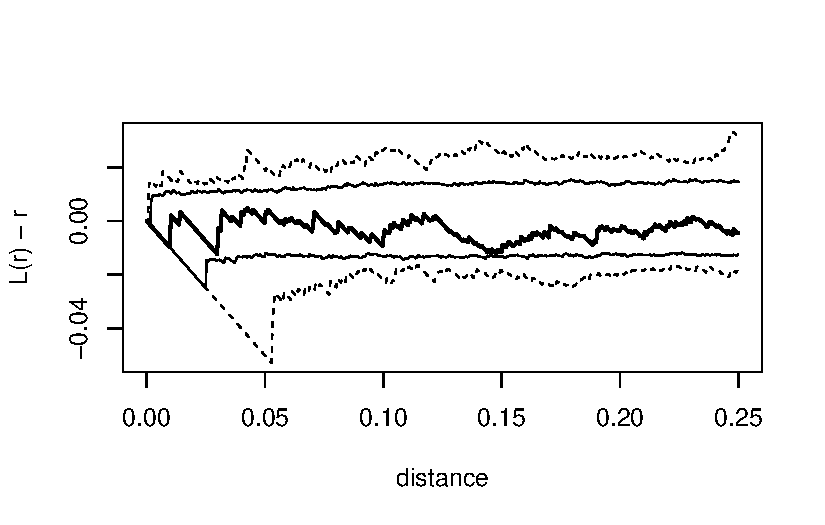
\includegraphics{robby_homework_2_files/figure-pdf/unnamed-chunk-3-1.pdf}

}

\end{figure}

\hypertarget{part-b.}{%
\subsubsection{Part b.}\label{part-b.}}

\begin{quote}
Based on the plot from part a, the Japanese Pines data appears
consistent with CSR across all spatial scales and no indication of
regularity or clustering.
\end{quote}

\hypertarget{part-c.}{%
\subsubsection{Part c.}\label{part-c.}}

\begin{Shaded}
\begin{Highlighting}[]
\NormalTok{win }\OtherTok{=}\NormalTok{ numata\_pines}\SpecialCharTok{$}\NormalTok{window}
\NormalTok{lambda }\OtherTok{=}\NormalTok{ numata\_pines}\SpecialCharTok{$}\NormalTok{n}


\NormalTok{lobserved }\OtherTok{\textless{}{-}}\NormalTok{ spatstat.explore}\SpecialCharTok{::}\FunctionTok{Lest}\NormalTok{(}\AttributeTok{X=}\NormalTok{numata\_pines, }\AttributeTok{correction =} \StringTok{"Ripley"}\NormalTok{)}
\NormalTok{lr }\OtherTok{=}\NormalTok{ lobserved}\SpecialCharTok{$}\NormalTok{iso}
\NormalTok{r }\OtherTok{=}\NormalTok{ lobserved}\SpecialCharTok{$}\NormalTok{r}
\NormalTok{tobs }\OtherTok{=} \FunctionTok{max}\NormalTok{(}\FunctionTok{abs}\NormalTok{(lr}\SpecialCharTok{{-}}\NormalTok{r))}

\NormalTok{lrl }\OtherTok{\textless{}{-}}\NormalTok{ pbapply}\SpecialCharTok{::}\FunctionTok{pbsapply}\NormalTok{(}\DecValTok{1}\SpecialCharTok{:}\DecValTok{499}\NormalTok{, }\AttributeTok{FUN =} \ControlFlowTok{function}\NormalTok{(i) \{}
\NormalTok{  xs }\OtherTok{\textless{}{-}}\NormalTok{ spatstat.random}\SpecialCharTok{::}\FunctionTok{rpoispp}\NormalTok{(}\AttributeTok{lambda =}\NormalTok{ lambda, }\AttributeTok{win =}\NormalTok{ win)}
  \FunctionTok{max}\NormalTok{(}\FunctionTok{abs}\NormalTok{(spatstat.explore}\SpecialCharTok{::}\FunctionTok{Lest}\NormalTok{(xs,}\AttributeTok{correction =} \StringTok{"Ripley"}\NormalTok{)}\SpecialCharTok{$}\NormalTok{iso}\SpecialCharTok{{-}}\NormalTok{r))}
  
\NormalTok{\})}

\FunctionTok{mean}\NormalTok{(}\FunctionTok{c}\NormalTok{(tobs,lrl)}\SpecialCharTok{\textgreater{}=}\NormalTok{tobs)}
\end{Highlighting}
\end{Shaded}

\begin{verbatim}
[1] 0.738
\end{verbatim}

\begin{quote}
The Monte Carlo p-value suggests that the Numata Pines data is
consistent with CSR since we fail to reject the null that our observed
test statistic and the simulated test statistic come from the same
distribution, and since the simulated distribution is consistent with
CSR by design.
\end{quote}

\hypertarget{problem-2}{%
\subsection{Problem 2}\label{problem-2}}

\hypertarget{part-a.-1}{%
\subsubsection{Part a.}\label{part-a.-1}}

\begin{Shaded}
\begin{Highlighting}[]
\NormalTok{redwood }\OtherTok{\textless{}{-}}\NormalTok{ spatstat.data}\SpecialCharTok{::}\NormalTok{redwood}
\FunctionTok{plot}\NormalTok{(redwood}\SpecialCharTok{$}\NormalTok{x,redwood}\SpecialCharTok{$}\NormalTok{y,}\AttributeTok{xlab=}\StringTok{\textquotesingle{}U\textquotesingle{}}\NormalTok{,}\AttributeTok{ylab=}\StringTok{\textquotesingle{}V\textquotesingle{}}\NormalTok{,}\AttributeTok{main=}\StringTok{\textquotesingle{}California Redwood Seedling/Sapling Locations\textquotesingle{}}\NormalTok{)}
\end{Highlighting}
\end{Shaded}

\begin{figure}[H]

{\centering 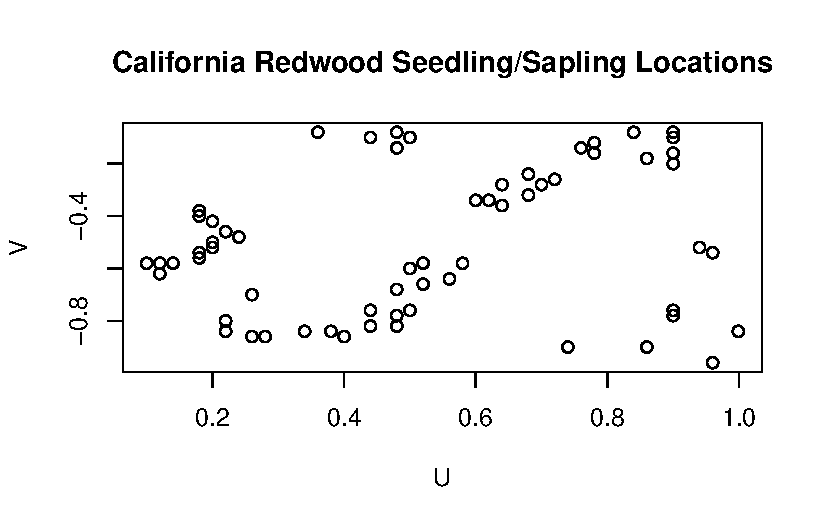
\includegraphics{robby_homework_2_files/figure-pdf/unnamed-chunk-5-1.pdf}

}

\end{figure}

\begin{quote}
At first glance, the distribution of seedling/sapling locations does not
appear to be consistent with CSR and we see some potential clustering.
\end{quote}

\hypertarget{part-b.-1}{%
\subsubsection{Part b.}\label{part-b.-1}}

\begin{Shaded}
\begin{Highlighting}[]
\NormalTok{dim }\OtherTok{=} \DecValTok{2}
\NormalTok{bx }\OtherTok{=} \FunctionTok{sd}\NormalTok{(redwood}\SpecialCharTok{$}\NormalTok{x)}\SpecialCharTok{*}\FunctionTok{length}\NormalTok{(redwood}\SpecialCharTok{$}\NormalTok{x)}\SpecialCharTok{\^{}}\NormalTok{(}\SpecialCharTok{{-}}\DecValTok{1}\SpecialCharTok{/}\NormalTok{(dim}\SpecialCharTok{+}\DecValTok{4}\NormalTok{))}
\NormalTok{by }\OtherTok{=} \FunctionTok{sd}\NormalTok{(redwood}\SpecialCharTok{$}\NormalTok{y)}\SpecialCharTok{*}\FunctionTok{length}\NormalTok{(redwood}\SpecialCharTok{$}\NormalTok{y)}\SpecialCharTok{\^{}}\NormalTok{(}\SpecialCharTok{{-}}\DecValTok{1}\SpecialCharTok{/}\NormalTok{(dim}\SpecialCharTok{+}\DecValTok{4}\NormalTok{))}

\NormalTok{ix }\OtherTok{=} \FunctionTok{density}\NormalTok{(redwood,}\AttributeTok{sigma =} \FunctionTok{c}\NormalTok{(bx,by))}
\FunctionTok{contour}\NormalTok{(ix}\SpecialCharTok{$}\NormalTok{v,}\AttributeTok{main=}\StringTok{\textquotesingle{}California Redwood Seedling/Sapling Contours\textquotesingle{}}\NormalTok{)}
\end{Highlighting}
\end{Shaded}

\begin{figure}[H]

{\centering 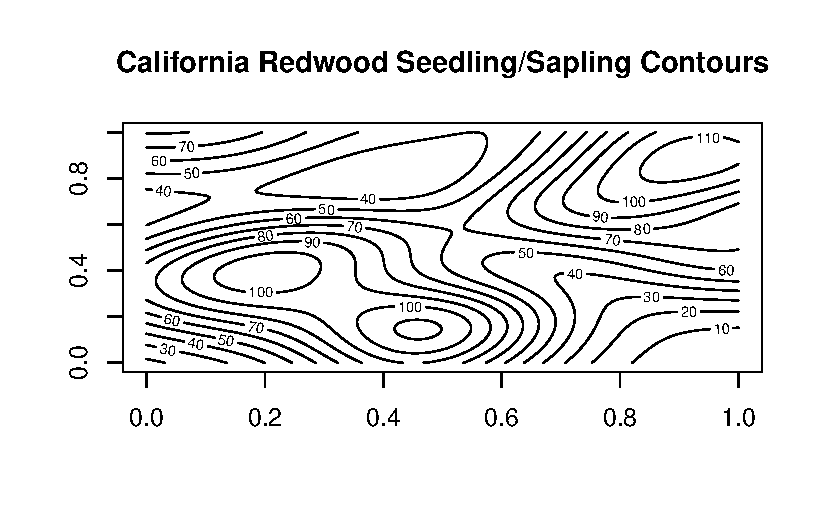
\includegraphics{robby_homework_2_files/figure-pdf/unnamed-chunk-6-1.pdf}

}

\end{figure}

\begin{quote}
Since the contours show areas of greater or lower intensity relative to
the rest of the study area, we would not think the underlying data to be
consistent with CSR.
\end{quote}

\hypertarget{part-c.-1}{%
\subsubsection{Part c.}\label{part-c.-1}}

\begin{Shaded}
\begin{Highlighting}[]
\FunctionTok{lplot}\NormalTok{(redwood)}
\end{Highlighting}
\end{Shaded}

\begin{figure}[H]

{\centering 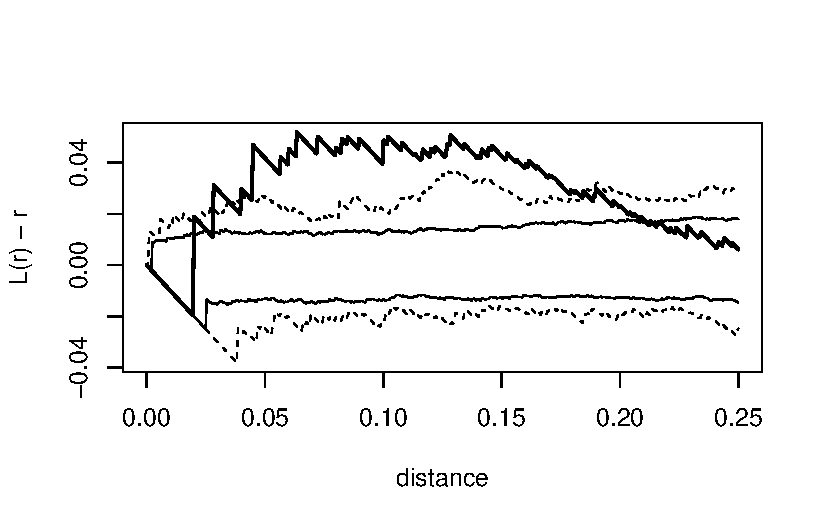
\includegraphics{robby_homework_2_files/figure-pdf/unnamed-chunk-7-1.pdf}

}

\end{figure}

\hypertarget{part-d.}{%
\subsubsection{Part d.}\label{part-d.}}

\begin{quote}
From the L(r) - r plot above we can see that there is evidence of
clustering beyond what we would expect for a point process compatible
with CSR for certain spatial scales up to about r=0.22.
\end{quote}

\hypertarget{part-e.}{%
\subsubsection{Part e.}\label{part-e.}}

\begin{Shaded}
\begin{Highlighting}[]
\NormalTok{win }\OtherTok{=}\NormalTok{ redwood}\SpecialCharTok{$}\NormalTok{window}
\NormalTok{lambda }\OtherTok{=}\NormalTok{ redwood}\SpecialCharTok{$}\NormalTok{n}


\NormalTok{lobserved }\OtherTok{\textless{}{-}}\NormalTok{ spatstat.explore}\SpecialCharTok{::}\FunctionTok{Lest}\NormalTok{(}\AttributeTok{X=}\NormalTok{redwood, }\AttributeTok{correction =} \StringTok{"Ripley"}\NormalTok{)}
\NormalTok{lr }\OtherTok{=}\NormalTok{ lobserved}\SpecialCharTok{$}\NormalTok{iso}
\NormalTok{r }\OtherTok{=}\NormalTok{ lobserved}\SpecialCharTok{$}\NormalTok{r}
\NormalTok{tobs }\OtherTok{=} \FunctionTok{max}\NormalTok{(}\FunctionTok{abs}\NormalTok{(lr}\SpecialCharTok{{-}}\NormalTok{r))}

\NormalTok{lrl }\OtherTok{\textless{}{-}}\NormalTok{ pbapply}\SpecialCharTok{::}\FunctionTok{pbsapply}\NormalTok{(}\DecValTok{1}\SpecialCharTok{:}\DecValTok{499}\NormalTok{, }\AttributeTok{FUN =} \ControlFlowTok{function}\NormalTok{(i) \{}
\NormalTok{  xs }\OtherTok{\textless{}{-}}\NormalTok{ spatstat.random}\SpecialCharTok{::}\FunctionTok{rpoispp}\NormalTok{(}\AttributeTok{lambda =}\NormalTok{ lambda, }\AttributeTok{win =}\NormalTok{ win)}
  \FunctionTok{max}\NormalTok{(}\FunctionTok{abs}\NormalTok{(spatstat.explore}\SpecialCharTok{::}\FunctionTok{Lest}\NormalTok{(xs,}\AttributeTok{correction =} \StringTok{"Ripley"}\NormalTok{)}\SpecialCharTok{$}\NormalTok{iso}\SpecialCharTok{{-}}\NormalTok{r))}
  
\NormalTok{\})}

\FunctionTok{mean}\NormalTok{(}\FunctionTok{c}\NormalTok{(tobs,lrl)}\SpecialCharTok{\textgreater{}=}\NormalTok{tobs)}
\end{Highlighting}
\end{Shaded}

\begin{verbatim}
[1] 0.002
\end{verbatim}

\begin{quote}
From the Monte-Carlo p-value calculated above we reject the null that
the observed statistic is from a distribution compatible with CSR.
\end{quote}

\hypertarget{part-f.}{%
\subsubsection{Part f.}\label{part-f.}}

\begin{quote}
Overall, there appears to be enough evidence to support the conclusion
that the Redwood sapling locations are not compatible with CSR and there
is more clustering than would be expected from a CSR point process.
\end{quote}

\hypertarget{problem-3}{%
\subsection{Problem 3}\label{problem-3}}

\begin{Shaded}
\begin{Highlighting}[]
\FunctionTok{set.seed}\NormalTok{(}\DecValTok{1}\NormalTok{)}
\NormalTok{x }\OtherTok{\textless{}{-}} \FunctionTok{runif}\NormalTok{(}\DecValTok{15}\NormalTok{)}

\NormalTok{h }\OtherTok{\textless{}{-}} \FunctionTok{seq}\NormalTok{(}\SpecialCharTok{{-}}\DecValTok{1}\NormalTok{,}\DecValTok{2}\NormalTok{,}\AttributeTok{len =} \DecValTok{1000}\NormalTok{)}
\end{Highlighting}
\end{Shaded}

\hypertarget{part-a.-2}{%
\subsubsection{Part a.}\label{part-a.-2}}

\begin{quote}
evaluate the Gaussian kernel function (dnorm) at each value of h using
the event location as the mean argument and a sd argument of 0.10
\end{quote}

\begin{Shaded}
\begin{Highlighting}[]
\NormalTok{kvals }\OtherTok{\textless{}{-}} \FunctionTok{data.frame}\NormalTok{()}
\ControlFlowTok{for}\NormalTok{ (i }\ControlFlowTok{in} \DecValTok{1}\SpecialCharTok{:}\DecValTok{1000}\NormalTok{)\{}
\NormalTok{  j }\OtherTok{=} \DecValTok{0}
  \ControlFlowTok{for}\NormalTok{ (xi }\ControlFlowTok{in}\NormalTok{ x)\{}
\NormalTok{    j }\OtherTok{=}\NormalTok{ j}\SpecialCharTok{+}\DecValTok{1}
\NormalTok{    kg }\OtherTok{=} \FunctionTok{dnorm}\NormalTok{(xi,}\AttributeTok{mean =}\NormalTok{ h[i], }\AttributeTok{sd=}\FloatTok{0.10}\NormalTok{)}
\NormalTok{    kvals[i,j] }\OtherTok{=}\NormalTok{ kg}
\NormalTok{  \}}

\NormalTok{\}}

\FunctionTok{str}\NormalTok{(kvals)}
\end{Highlighting}
\end{Shaded}

\begin{verbatim}
'data.frame':   1000 obs. of  15 variables:
 $ V1 : num  6.68e-35 9.76e-35 1.43e-34 2.08e-34 3.03e-34 ...
 $ V2 : num  5.22e-41 7.89e-41 1.19e-40 1.79e-40 2.70e-40 ...
 $ V3 : num  7.61e-54 1.22e-53 1.95e-53 3.13e-53 5.00e-53 ...
 $ V4 : num  3.40e-79 6.04e-79 1.07e-78 1.89e-78 3.34e-78 ...
 $ V5 : num  1.75e-31 2.51e-31 3.60e-31 5.16e-31 7.37e-31 ...
 $ V6 : num  2.21e-78 3.90e-78 6.89e-78 1.21e-77 2.14e-77 ...
 $ V7 : num  3.03e-82 5.43e-82 9.72e-82 1.74e-81 3.11e-81 ...
 $ V8 : num  5.08e-60 8.37e-60 1.38e-59 2.26e-59 3.71e-59 ...
 $ V9 : num  9.33e-58 1.52e-57 2.48e-57 4.03e-57 6.55e-57 ...
 $ V10: num  1.32e-24 1.81e-24 2.49e-24 3.42e-24 4.69e-24 ...
 $ V11: num  1.05e-31 1.50e-31 2.15e-31 3.09e-31 4.42e-31 ...
 $ V12: num  3.48e-30 4.95e-30 7.04e-30 1.00e-29 1.42e-29 ...
 $ V13: num  6.31e-62 1.05e-61 1.73e-61 2.87e-61 4.75e-61 ...
 $ V14: num  1.00e-41 1.52e-41 2.30e-41 3.47e-41 5.25e-41 ...
 $ V15: num  3.83e-68 6.51e-68 1.11e-67 1.88e-67 3.19e-67 ...
\end{verbatim}

\begin{Shaded}
\begin{Highlighting}[]
\NormalTok{kval\_totals }\OtherTok{\textless{}{-}} \FunctionTok{pbapply}\NormalTok{(kvals,}\AttributeTok{MARGIN=}\DecValTok{1}\NormalTok{,}\AttributeTok{FUN=}\StringTok{\textquotesingle{}sum\textquotesingle{}}\NormalTok{)}

\FunctionTok{plot}\NormalTok{(h,kval\_totals)}
\end{Highlighting}
\end{Shaded}

\begin{figure}[H]

{\centering 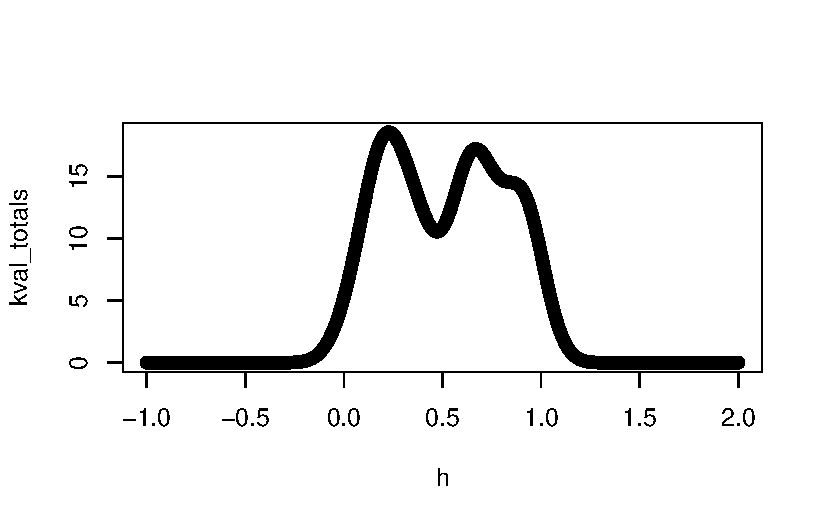
\includegraphics{robby_homework_2_files/figure-pdf/unnamed-chunk-10-1.pdf}

}

\end{figure}

Part b.

\begin{quote}
Repeat using sd/bandwidth of 0.25
\end{quote}

\begin{Shaded}
\begin{Highlighting}[]
\NormalTok{kvals }\OtherTok{\textless{}{-}} \FunctionTok{data.frame}\NormalTok{()}
\ControlFlowTok{for}\NormalTok{ (i }\ControlFlowTok{in} \DecValTok{1}\SpecialCharTok{:}\DecValTok{1000}\NormalTok{)\{}
\NormalTok{  j }\OtherTok{=} \DecValTok{0}
  \ControlFlowTok{for}\NormalTok{ (xi }\ControlFlowTok{in}\NormalTok{ x)\{}
\NormalTok{    j }\OtherTok{=}\NormalTok{ j}\SpecialCharTok{+}\DecValTok{1}
\NormalTok{    kg }\OtherTok{=} \FunctionTok{dnorm}\NormalTok{(xi,}\AttributeTok{mean =}\NormalTok{ h[i], }\AttributeTok{sd=}\NormalTok{.}\DecValTok{25}\NormalTok{)}
\NormalTok{    kvals[i,j] }\OtherTok{=}\NormalTok{ kg}
\NormalTok{  \}}

\NormalTok{\}}

\FunctionTok{str}\NormalTok{(kvals)}
\end{Highlighting}
\end{Shaded}

\begin{verbatim}
'data.frame':   1000 obs. of  15 variables:
 $ V1 : num  4.35e-06 4.63e-06 4.91e-06 5.22e-06 5.54e-06 ...
 $ V2 : num  4.59e-07 4.90e-07 5.23e-07 5.59e-07 5.97e-07 ...
 $ V3 : num  4.05e-09 4.37e-09 4.71e-09 5.08e-09 5.48e-09 ...
 $ V4 : num  3.56e-13 3.91e-13 4.28e-13 4.69e-13 5.14e-13 ...
 $ V5 : num  1.53e-05 1.63e-05 1.72e-05 1.82e-05 1.93e-05 ...
 $ V6 : num  4.81e-13 5.26e-13 5.77e-13 6.31e-13 6.91e-13 ...
 $ V7 : num  1.16e-13 1.27e-13 1.40e-13 1.53e-13 1.68e-13 ...
 $ V8 : num  4.17e-10 4.51e-10 4.89e-10 5.29e-10 5.73e-10 ...
 $ V9 : num  9.59e-10 1.04e-09 1.12e-09 1.21e-09 1.31e-09 ...
 $ V10: num  0.000193 0.000203 0.000214 0.000225 0.000237 ...
 $ V11: num  1.41e-05 1.50e-05 1.59e-05 1.68e-05 1.78e-05 ...
 $ V12: num  2.47e-05 2.62e-05 2.77e-05 2.93e-05 3.10e-05 ...
 $ V13: num  2.06e-10 2.24e-10 2.43e-10 2.63e-10 2.85e-10 ...
 $ V14: num  3.52e-07 3.77e-07 4.02e-07 4.30e-07 4.59e-07 ...
 $ V15: num  2.09e-11 2.28e-11 2.48e-11 2.70e-11 2.93e-11 ...
\end{verbatim}

\begin{Shaded}
\begin{Highlighting}[]
\NormalTok{kval\_totals }\OtherTok{\textless{}{-}} \FunctionTok{pbapply}\NormalTok{(kvals,}\AttributeTok{MARGIN=}\DecValTok{1}\NormalTok{,}\AttributeTok{FUN=}\StringTok{\textquotesingle{}sum\textquotesingle{}}\NormalTok{)}

\FunctionTok{plot}\NormalTok{(h,kval\_totals)}
\end{Highlighting}
\end{Shaded}

\begin{figure}[H]

{\centering 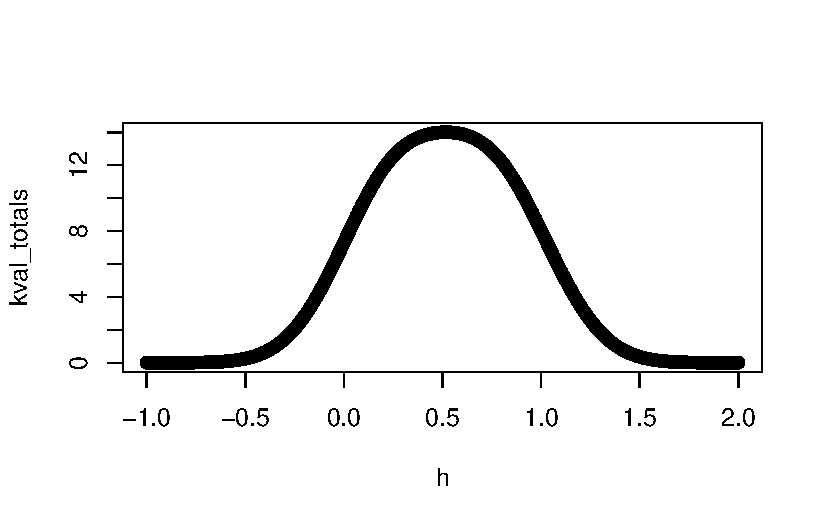
\includegraphics{robby_homework_2_files/figure-pdf/unnamed-chunk-11-1.pdf}

}

\end{figure}

Part c.

\begin{quote}
The relationship between the bandwidth and the smoothness of the density
function is that a larger bandwidth gives a smoother density function.
\end{quote}



\end{document}
